
\chapter{FOB Formalism}
\label{chap:FOB}
The effect of the nuclei on the electrons is normally handled via the Hamiltonian. This is dependent on nuclear positions and is in turn used in the Schr\"odinger equation to propagate the electron dynamics. Often the construction of the Hamiltonian is carried out using density function theory (DFT). However, for large, dynamic systems this becomes too computationally expensive and a different technique should be used. In this work I will rely on an Analytical Overlap Method (AOM) \cite{gajdos_ultrafast_2014} to calculate the off-diagonal elements of the Hamiltonian. The diagonal elements will be calculated via a forcefield.
\section{AOM}
\begin{wrapfigure}{r}{0.45\textwidth}
  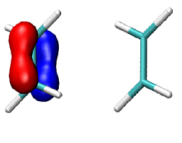
\includegraphics[width=0.45\textwidth]{./img/SOMO.png}
  \caption{\label{fig:SOMO}A depiction of a singly occupied molecular orbital (SOMO) on an ethylene molecule. Adapted from \cite{spencer_fob-sh:_2016}.}
\end{wrapfigure}
AOM assumes that the off-diagonal elements of the Hamiltonian are proportional to the off-diagonal elements of the overlap matrix between 2 singly occupied molecular orbitals (SOMO) see figure \ref{fig:SOMO}. This is show in equation \eqref{eq:H-CS}.
\begin{equation}
    H_{kl} = C S_{kl}
    \label{eq:H-CS}
\end{equation}
This approximation was originally by Longuet-Higgins and Roberts \cite{Prezhdo1997Oct} and its validity has been tested in our group previously in the small overlap regime \cite{gajdos_ultrafast_2014}.  Many of the presently most studied and promising organic semiconductors, such as Rubrene \cite{Braga2009Feb,Baris2014Aug} and Pentacene \cite{Tiwari2010May, Kim2015Dec} have pi-conjugation. In these systems it is often sufficient to include only 1 optimised p-orbital per atom
\cite{spencer_fob-sh:_2016}. This gives us an equation for the overlap of the SOMOs ($\varphi_{k}$) as:
\begin{equation}
    S_{kl}^{'} = \langle \varphi_{k} | \varphi_{l} \rangle = \sum_{i \in k}^{atoms} \sum_{j \in l}^{atoms} c_{p\pi, i}^{*} c_{p\pi, j} \langle p_{\pi, i}|p_{\pi, j}\rangle
    \label{eq:P-orbital-overlap}
\end{equation}
Where $\langle p_{\pi, i} |$ represents the optimised Slater p-orbital and the $c_{p\pi, i}$ terms are the AOM expansion coefficients. The gradient of the Hamiltonian can also be expressed in terms of the gradient of the overlap $\nabla_{\nu} H_{kl} = C \nabla_{\nu} S_{kl}$ (where $\nu$ represents the atom index). Further efficiencies can be made by expressing the gradient of the overlap in terms of (diabatic) NACVs e.g:
\begin{equation}
  \nabla_{\nu} H_{kl}^{'} = C \ \nabla_{\nu} S_{kl}^{'} = C \ \nabla_{\nu} \langle \varphi_{k} | \varphi_{l} \rangle = C ( \textbf{d}_{\nu, lk}^{'*} + \textbf{d}_{\nu, kl}^{'} )
\end{equation}
Where we have defined the non-adiabatic coupling vectors (in a non-orthogonal diabtic basis) as $\textbf{d}^{'}_{\nu, lk} = \langle \varphi_{l}  | \nabla_{\nu} \varphi_{k}\rangle$. The $H^{'}_{kl}$ term is the Hamiltonian in the non-orthogonal diabatic basis. The NACVs are calculated via a fintie difference method.

\section{Different Bases}
The definitions in the previous section giving the key points in the AOM method were all expressed in a non-orthogonal diabatic basis. However, the electronic propagation in the FOB method is done in an orthogonal diabatic basis denoted $\phi_{l}$. Further the CTMQC equations have been derived and are expressed in the adiabtic basis, $\psi_{l}$. Therefore, it is important to define the transformations between the 3 bases used in the code.
\subsubsection{Basis Expansion}
The time-dependent electronic wavefunction can be expressed as a linear combination of basis functions with expansion coefficients determining the size of their contribution. For example:
\begin{equation}
  \Phi_{\textbf{R}}(\textbf{r}, t) = \sum_{n}^{N_{states}}C_{n}(\textbf{R}, t) \psi_{\textbf{R}, n}(\textbf{r}) = \sum_{l}^{N_{states}} u_{l}(\textbf{R}, t) \phi_{\textbf{R}, l}(\textbf{r})
\end{equation}
Where $\Phi_{\textbf{R}}(\textbf{r}, t)$ is the electronic wavefunction in the exact factorisation formalism. The subscript $\textbf{R}$ denotes a parametric dependence on nuclear coordinates, the subscript $n$ denote adiabatic state n similarly $l$ denotes the l$^{th}$ (orthogonal) diabatic state. Throughout this document I will use the following naming convention: $\textbf{R}$ denotes nuclear coordinates and $\textbf{r}$ for the electronic coordinates. The $C_{l}$ is the l$^{th}$ adiabatic state. The squared modulus of this gives the population of electrons on that state. Expressing the electronic wavefunction in this way allows us to rewrite the propagation equations in terms of the expansion coefficients $C_{l}$ or $u_{l}$.
\\\\
As the propagation equations are written in terms of the expansion coefficients it is sensible to give the transformation equation in terms of them. To transform from the adiabatic to diabatic basis we can use the following unitary transformation:
\begin{equation}
  \vec{C}(\textbf{R}, t) = \mathbb{U}(\textbf{R}, t) \  \vec{u}(\textbf{R}, t)
  \label{eq:ad_to_di}
\end{equation}
Here we have expressed the expansion coefficients as a vector e.g. $\vec{C} = \left( \begin{array}{c}
C_1 \\
\vdots \\
C_n
\end{array}\right)$
The unitary transformation matrix is given as the overlap between diabatic and adiabatic states, $U_{ln} = \langle \phi_{l} | \psi_{n} \rangle$, and is a square matrix of size $N_{states}^2$. This is obtained by diagonalising the Hamiltonian in the code. The fact that this matrix is unitary means transforming from the diabatic to adiabatic is no more computationally expensive. The transformation can be obtained by pre-multiplying both sides of eq \eqref{eq:ad_to_di} by $\mathbb{U}^{\dagger}$ e.g.
\begin{equation}
  \mathbb{U}^{\dagger}(\textbf{R}, t) \vec{C}(\textbf{R}, t) = \vec{u}(\textbf{R}, t)
  \label{eq:diab_to_adiab}
\end{equation}
\\\\
To trasform from the non-orthogonal to orthogonal basis we need a new matrix. This is given by:
\begin{equation}
  \vec{\phi} = \mathbb{T} \vec{\varphi}
  \label{eq:orth_to_nonorth}
\end{equation}
This transformation is needed when transforming the non-orthogonal diabatic Hamiltonian, $H^{'}$, and non-adiabatic coupling terms to the orthogonal diabatic basis. For example, the orthogonal diabatic Hamiltonian is calculated as $H_{kl} = \left[\mathbb{T}^{-1} \mathbb{H}^{'} \mathbb{T} \right]_{kl}$. This matrix is equal to the inverse square of the overlap between SOMOs i.e. $T_{ml} = [\mathbb{S}^{-\frac{1}{2}}]_{ml}$.
\\\\
Replacing the full charge transfer determinant with parametrised singly occupied molecular orbitals (SOMOs) makes the calculation of the relevant terms in the propagation of the system very efficient. The approximation has been scrutinised before in the group
\cite{giannini_crossover_2018, carof_detailed_2017, gajdos_ultrafast_2014, Gajdos2013Mar, spencer_confronting_2016, spencer_fob-sh:_2016} and its first implementation within the surface hopping framework has been shown to reproduce known phenomena such as the crossover from band-like to hopping-like transport \cite{giannini_crossover_2018}. In this way the interaction of the nuclei on the electrons is accounted for, as the overlap between SOMOs (and therefore the coupling, $H_{ab}$) depends on the nuclear geometry.
